% Options for packages loaded elsewhere
\PassOptionsToPackage{unicode}{hyperref}
\PassOptionsToPackage{hyphens}{url}
%
\documentclass[
]{article}
\usepackage{lmodern}
\usepackage{amssymb,amsmath}
\usepackage{ifxetex,ifluatex}
\ifnum 0\ifxetex 1\fi\ifluatex 1\fi=0 % if pdftex
  \usepackage[T1]{fontenc}
  \usepackage[utf8]{inputenc}
  \usepackage{textcomp} % provide euro and other symbols
\else % if luatex or xetex
  \usepackage{unicode-math}
  \defaultfontfeatures{Scale=MatchLowercase}
  \defaultfontfeatures[\rmfamily]{Ligatures=TeX,Scale=1}
\fi
% Use upquote if available, for straight quotes in verbatim environments
\IfFileExists{upquote.sty}{\usepackage{upquote}}{}
\IfFileExists{microtype.sty}{% use microtype if available
  \usepackage[]{microtype}
  \UseMicrotypeSet[protrusion]{basicmath} % disable protrusion for tt fonts
}{}
\makeatletter
\@ifundefined{KOMAClassName}{% if non-KOMA class
  \IfFileExists{parskip.sty}{%
    \usepackage{parskip}
  }{% else
    \setlength{\parindent}{0pt}
    \setlength{\parskip}{6pt plus 2pt minus 1pt}}
}{% if KOMA class
  \KOMAoptions{parskip=half}}
\makeatother
\usepackage{xcolor}
\IfFileExists{xurl.sty}{\usepackage{xurl}}{} % add URL line breaks if available
\IfFileExists{bookmark.sty}{\usepackage{bookmark}}{\usepackage{hyperref}}
\hypersetup{
  pdftitle={06 Map},
  pdfauthor={Thomas J. Brailey},
  hidelinks,
  pdfcreator={LaTeX via pandoc}}
\urlstyle{same} % disable monospaced font for URLs
\usepackage[margin=1in]{geometry}
\usepackage{color}
\usepackage{fancyvrb}
\newcommand{\VerbBar}{|}
\newcommand{\VERB}{\Verb[commandchars=\\\{\}]}
\DefineVerbatimEnvironment{Highlighting}{Verbatim}{commandchars=\\\{\}}
% Add ',fontsize=\small' for more characters per line
\usepackage{framed}
\definecolor{shadecolor}{RGB}{248,248,248}
\newenvironment{Shaded}{\begin{snugshade}}{\end{snugshade}}
\newcommand{\AlertTok}[1]{\textcolor[rgb]{0.94,0.16,0.16}{#1}}
\newcommand{\AnnotationTok}[1]{\textcolor[rgb]{0.56,0.35,0.01}{\textbf{\textit{#1}}}}
\newcommand{\AttributeTok}[1]{\textcolor[rgb]{0.77,0.63,0.00}{#1}}
\newcommand{\BaseNTok}[1]{\textcolor[rgb]{0.00,0.00,0.81}{#1}}
\newcommand{\BuiltInTok}[1]{#1}
\newcommand{\CharTok}[1]{\textcolor[rgb]{0.31,0.60,0.02}{#1}}
\newcommand{\CommentTok}[1]{\textcolor[rgb]{0.56,0.35,0.01}{\textit{#1}}}
\newcommand{\CommentVarTok}[1]{\textcolor[rgb]{0.56,0.35,0.01}{\textbf{\textit{#1}}}}
\newcommand{\ConstantTok}[1]{\textcolor[rgb]{0.00,0.00,0.00}{#1}}
\newcommand{\ControlFlowTok}[1]{\textcolor[rgb]{0.13,0.29,0.53}{\textbf{#1}}}
\newcommand{\DataTypeTok}[1]{\textcolor[rgb]{0.13,0.29,0.53}{#1}}
\newcommand{\DecValTok}[1]{\textcolor[rgb]{0.00,0.00,0.81}{#1}}
\newcommand{\DocumentationTok}[1]{\textcolor[rgb]{0.56,0.35,0.01}{\textbf{\textit{#1}}}}
\newcommand{\ErrorTok}[1]{\textcolor[rgb]{0.64,0.00,0.00}{\textbf{#1}}}
\newcommand{\ExtensionTok}[1]{#1}
\newcommand{\FloatTok}[1]{\textcolor[rgb]{0.00,0.00,0.81}{#1}}
\newcommand{\FunctionTok}[1]{\textcolor[rgb]{0.00,0.00,0.00}{#1}}
\newcommand{\ImportTok}[1]{#1}
\newcommand{\InformationTok}[1]{\textcolor[rgb]{0.56,0.35,0.01}{\textbf{\textit{#1}}}}
\newcommand{\KeywordTok}[1]{\textcolor[rgb]{0.13,0.29,0.53}{\textbf{#1}}}
\newcommand{\NormalTok}[1]{#1}
\newcommand{\OperatorTok}[1]{\textcolor[rgb]{0.81,0.36,0.00}{\textbf{#1}}}
\newcommand{\OtherTok}[1]{\textcolor[rgb]{0.56,0.35,0.01}{#1}}
\newcommand{\PreprocessorTok}[1]{\textcolor[rgb]{0.56,0.35,0.01}{\textit{#1}}}
\newcommand{\RegionMarkerTok}[1]{#1}
\newcommand{\SpecialCharTok}[1]{\textcolor[rgb]{0.00,0.00,0.00}{#1}}
\newcommand{\SpecialStringTok}[1]{\textcolor[rgb]{0.31,0.60,0.02}{#1}}
\newcommand{\StringTok}[1]{\textcolor[rgb]{0.31,0.60,0.02}{#1}}
\newcommand{\VariableTok}[1]{\textcolor[rgb]{0.00,0.00,0.00}{#1}}
\newcommand{\VerbatimStringTok}[1]{\textcolor[rgb]{0.31,0.60,0.02}{#1}}
\newcommand{\WarningTok}[1]{\textcolor[rgb]{0.56,0.35,0.01}{\textbf{\textit{#1}}}}
\usepackage{graphicx,grffile}
\makeatletter
\def\maxwidth{\ifdim\Gin@nat@width>\linewidth\linewidth\else\Gin@nat@width\fi}
\def\maxheight{\ifdim\Gin@nat@height>\textheight\textheight\else\Gin@nat@height\fi}
\makeatother
% Scale images if necessary, so that they will not overflow the page
% margins by default, and it is still possible to overwrite the defaults
% using explicit options in \includegraphics[width, height, ...]{}
\setkeys{Gin}{width=\maxwidth,height=\maxheight,keepaspectratio}
% Set default figure placement to htbp
\makeatletter
\def\fps@figure{htbp}
\makeatother
\setlength{\emergencystretch}{3em} % prevent overfull lines
\providecommand{\tightlist}{%
  \setlength{\itemsep}{0pt}\setlength{\parskip}{0pt}}
\setcounter{secnumdepth}{-\maxdimen} % remove section numbering

\title{06 Map}
\author{Thomas J. Brailey}
\date{1/24/2020}

\begin{document}
\maketitle

{
\setcounter{tocdepth}{2}
\tableofcontents
}
\hypertarget{load-data}{%
\section{Load data}\label{load-data}}

\begin{Shaded}
\begin{Highlighting}[]
\NormalTok{mali <-}\StringTok{ }\NormalTok{sf}\OperatorTok{::}\KeywordTok{st_read}\NormalTok{(}\KeywordTok{paste0}\NormalTok{(here}\OperatorTok{::}\KeywordTok{here}\NormalTok{(), }\StringTok{"/data/map/gadm36_MLI_shp/gadm36_MLI_0.shp"}\NormalTok{))}
\end{Highlighting}
\end{Shaded}

\begin{verbatim}
## Reading layer `gadm36_MLI_0' from data source `C:\Users\tbrai\Dropbox\github_private\SeniorThesis\data\map\gadm36_MLI_shp\gadm36_MLI_0.shp' using driver `ESRI Shapefile'
## Simple feature collection with 1 feature and 2 fields
## geometry type:  POLYGON
## dimension:      XY
## bbox:           xmin: -12.23891 ymin: 10.15951 xmax: 4.244968 ymax: 25
## epsg (SRID):    4326
## proj4string:    +proj=longlat +datum=WGS84 +no_defs
\end{verbatim}

\begin{Shaded}
\begin{Highlighting}[]
\NormalTok{niger <-}\StringTok{ }\NormalTok{sf}\OperatorTok{::}\KeywordTok{st_read}\NormalTok{(}\KeywordTok{paste0}\NormalTok{(here}\OperatorTok{::}\KeywordTok{here}\NormalTok{(), }\StringTok{"/data/map/gadm36_NER_shp/gadm36_NER_0.shp"}\NormalTok{))}
\end{Highlighting}
\end{Shaded}

\begin{verbatim}
## Reading layer `gadm36_NER_0' from data source `C:\Users\tbrai\Dropbox\github_private\SeniorThesis\data\map\gadm36_NER_shp\gadm36_NER_0.shp' using driver `ESRI Shapefile'
## Simple feature collection with 1 feature and 2 fields
## geometry type:  POLYGON
## dimension:      XY
## bbox:           xmin: 0.16625 ymin: 11.69697 xmax: 15.99564 ymax: 23.52503
## epsg (SRID):    4326
## proj4string:    +proj=longlat +datum=WGS84 +no_defs
\end{verbatim}

\begin{Shaded}
\begin{Highlighting}[]
\NormalTok{tuareg <-}\StringTok{ }\NormalTok{sf}\OperatorTok{::}\KeywordTok{st_read}\NormalTok{(}\KeywordTok{paste0}\NormalTok{(here}\OperatorTok{::}\KeywordTok{here}\NormalTok{(), }\StringTok{"/data/map/GeoEPR-2019/GeoEPR.shp"}\NormalTok{)) }\OperatorTok
\StringTok{  }\NormalTok{dplyr}\OperatorTok{::}\KeywordTok{filter}\NormalTok{(group }\OperatorTok{==}\StringTok{ "Tuareg"} \OperatorTok{&}\StringTok{ }
\StringTok{                  }\NormalTok{statename }\OperatorTok\StringTok{ }\KeywordTok{c}\NormalTok{(}\StringTok{"Mali"}\NormalTok{, }\StringTok{"Niger"}\NormalTok{) }\OperatorTok{&}\StringTok{ }
\StringTok{                  }\NormalTok{from }\OperatorTok{==}\StringTok{ }\DecValTok{1960}\NormalTok{)}
\end{Highlighting}
\end{Shaded}

\begin{verbatim}
## Reading layer `GeoEPR' from data source `C:\Users\tbrai\Dropbox\github_private\SeniorThesis\data\map\GeoEPR-2019\GeoEPR.shp' using driver `ESRI Shapefile'
## replacing null geometries with empty geometries
## Simple feature collection with 1470 features and 10 fields (with 134 geometries empty)
## geometry type:  GEOMETRY
## dimension:      XY
## bbox:           xmin: -180 ymin: -55.31195 xmax: 180 ymax: 76.99887
## epsg (SRID):    4326
## proj4string:    +proj=longlat +ellps=WGS84 +no_defs
\end{verbatim}

\begin{Shaded}
\begin{Highlighting}[]
\NormalTok{africa <-}\StringTok{ }\NormalTok{sf}\OperatorTok{::}\KeywordTok{st_read}\NormalTok{(}\KeywordTok{paste0}\NormalTok{(here}\OperatorTok{::}\KeywordTok{here}\NormalTok{(), }\StringTok{"/data/map/Africa_SHP/Africa.shp"}\NormalTok{))}
\end{Highlighting}
\end{Shaded}

\begin{verbatim}
## Reading layer `Africa' from data source `C:\Users\tbrai\Dropbox\github_private\SeniorThesis\data\map\Africa_SHP\Africa.shp' using driver `ESRI Shapefile'
## Simple feature collection with 762 features and 3 fields
## geometry type:  POLYGON
## dimension:      XY
## bbox:           xmin: -25.35875 ymin: -46.97893 xmax: 51.41303 ymax: 37.34962
## epsg (SRID):    NA
## proj4string:    NA
\end{verbatim}

\begin{Shaded}
\begin{Highlighting}[]
\NormalTok{sf}\OperatorTok{::}\KeywordTok{st_crs}\NormalTok{(africa) <-}\StringTok{ }\DecValTok{4326}
\end{Highlighting}
\end{Shaded}

\hypertarget{plot}{%
\section{Plot}\label{plot}}

\begin{Shaded}
\begin{Highlighting}[]
\NormalTok{map <-}\StringTok{ }\KeywordTok{ggplot}\NormalTok{() }\OperatorTok{+}
\StringTok{  }\KeywordTok{geom_sf}\NormalTok{(}\DataTypeTok{data =}\NormalTok{ tuareg, }\DataTypeTok{fill =} \StringTok{"#e6d073"}\NormalTok{, }\KeywordTok{aes}\NormalTok{(}\DataTypeTok{color =} \StringTok{"Tuareg Region"}\NormalTok{), }\DataTypeTok{alpha =} \FloatTok{.7}\NormalTok{) }\OperatorTok{+}
\StringTok{  }\KeywordTok{geom_sf}\NormalTok{(}\DataTypeTok{data =}\NormalTok{ africa, }\DataTypeTok{color =} \StringTok{"gray"}\NormalTok{, }\DataTypeTok{fill =} \StringTok{"hollow"}\NormalTok{) }\OperatorTok{+}
\StringTok{  }\KeywordTok{geom_sf}\NormalTok{(}\DataTypeTok{data =}\NormalTok{ mali, }\DataTypeTok{color =} \StringTok{"black"}\NormalTok{, }\DataTypeTok{fill =} \StringTok{"hollow"}\NormalTok{) }\OperatorTok{+}
\StringTok{  }\KeywordTok{geom_sf}\NormalTok{(}\DataTypeTok{data =}\NormalTok{ niger, }\DataTypeTok{color =} \StringTok{"black"}\NormalTok{, }\DataTypeTok{fill =} \StringTok{"hollow"}\NormalTok{) }\OperatorTok{+}
\StringTok{  }\KeywordTok{geom_sf_label}\NormalTok{(}\DataTypeTok{data =}\NormalTok{ mali, }\KeywordTok{aes}\NormalTok{(}\DataTypeTok{label =}\NormalTok{ NAME_}\DecValTok{0}\NormalTok{), }\DataTypeTok{fill =} \StringTok{"hollow"}\NormalTok{) }\OperatorTok{+}
\StringTok{  }\KeywordTok{geom_sf_label}\NormalTok{(}\DataTypeTok{data =}\NormalTok{ niger, }\KeywordTok{aes}\NormalTok{(}\DataTypeTok{label =}\NormalTok{ NAME_}\DecValTok{0}\NormalTok{), }\DataTypeTok{fill =} \StringTok{"hollow"}\NormalTok{) }\OperatorTok{+}
\StringTok{  }\KeywordTok{scale_color_manual}\NormalTok{(}\DataTypeTok{values =} \StringTok{"#e6d073"}\NormalTok{) }\OperatorTok{+}
\StringTok{  }\KeywordTok{labs}\NormalTok{(}\DataTypeTok{color =} \StringTok{""}\NormalTok{) }\OperatorTok{+}
\StringTok{  }\KeywordTok{coord_sf}\NormalTok{(}\DataTypeTok{xlim =} \KeywordTok{c}\NormalTok{(}\OperatorTok{-}\DecValTok{16}\NormalTok{, }\DecValTok{20}\NormalTok{), }\DataTypeTok{ylim =} \KeywordTok{c}\NormalTok{(}\DecValTok{8}\NormalTok{, }\DecValTok{26}\NormalTok{)) }\OperatorTok{+}
\StringTok{  }\KeywordTok{theme}\NormalTok{(}\DataTypeTok{axis.line=}\KeywordTok{element_blank}\NormalTok{(),}
          \DataTypeTok{axis.text.x=}\KeywordTok{element_blank}\NormalTok{(),}
          \DataTypeTok{axis.text.y=}\KeywordTok{element_blank}\NormalTok{(),}
          \DataTypeTok{axis.ticks=}\KeywordTok{element_blank}\NormalTok{(),}
          \DataTypeTok{axis.title.x=}\KeywordTok{element_blank}\NormalTok{(),}
          \DataTypeTok{axis.title.y=}\KeywordTok{element_blank}\NormalTok{(),   }
          \DataTypeTok{panel.border =} \KeywordTok{element_rect}\NormalTok{(}\DataTypeTok{colour =} \StringTok{"black"}\NormalTok{, }\DataTypeTok{fill=}\OtherTok{NA}\NormalTok{, }\DataTypeTok{size=}\DecValTok{1}\NormalTok{),}
          \DataTypeTok{panel.background=}\KeywordTok{element_blank}\NormalTok{(), }
          \DataTypeTok{panel.grid.major=}\KeywordTok{element_blank}\NormalTok{(),}
          \DataTypeTok{panel.grid.minor=}\KeywordTok{element_blank}\NormalTok{(),}
          \DataTypeTok{plot.background=}\KeywordTok{element_blank}\NormalTok{()) }
\NormalTok{map}
\end{Highlighting}
\end{Shaded}

\begin{verbatim}
## Warning in st_point_on_surface.sfc(sf::st_zm(x)): st_point_on_surface may not
## give correct results for longitude/latitude data

## Warning in st_point_on_surface.sfc(sf::st_zm(x)): st_point_on_surface may not
## give correct results for longitude/latitude data
\end{verbatim}

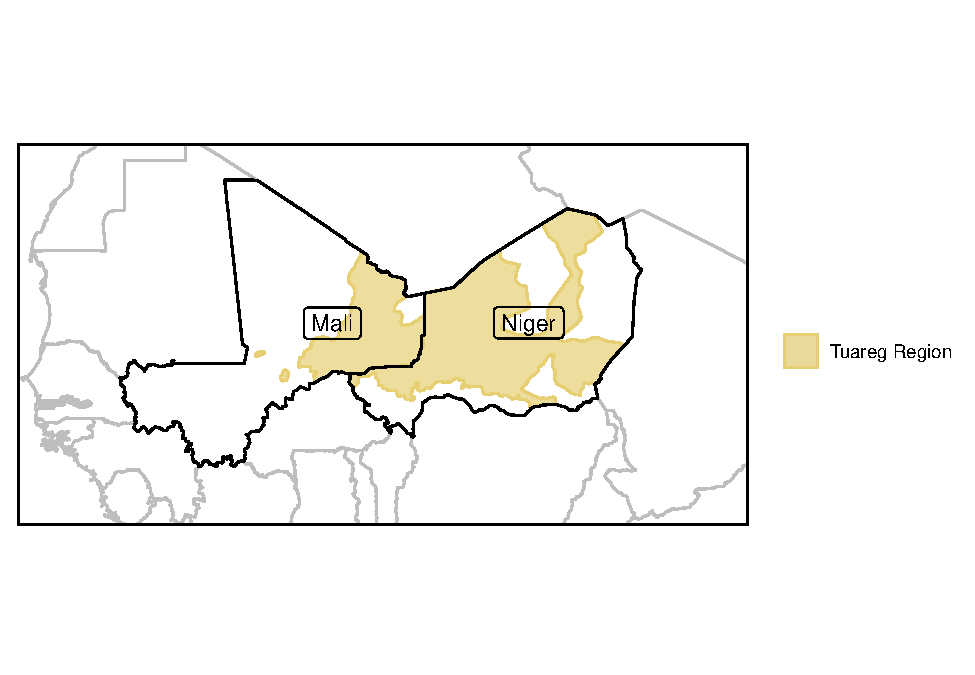
\includegraphics{06_tjbrailey_map_files/figure-latex/unnamed-chunk-2-1.pdf}

\hypertarget{save-data}{%
\section{Save data}\label{save-data}}

\begin{Shaded}
\begin{Highlighting}[]
\KeywordTok{ggsave}\NormalTok{(}\DataTypeTok{plot =}\NormalTok{ map, }\DataTypeTok{filename =} \KeywordTok{paste0}\NormalTok{(here}\OperatorTok{::}\KeywordTok{here}\NormalTok{(), }\StringTok{"/paper/tuareg_map.jpeg"}\NormalTok{), }\DataTypeTok{width =} \DecValTok{10}\NormalTok{, }\DataTypeTok{height =} \DecValTok{10}\NormalTok{)}
\end{Highlighting}
\end{Shaded}

\begin{verbatim}
## Warning in st_point_on_surface.sfc(sf::st_zm(x)): st_point_on_surface may not
## give correct results for longitude/latitude data

## Warning in st_point_on_surface.sfc(sf::st_zm(x)): st_point_on_surface may not
## give correct results for longitude/latitude data
\end{verbatim}

\end{document}
